\subsection{Management Pages}

\noindent These pages are designed for administrators and supervisors to oversee the academic and operational aspects of the platform.

\subsubsection{Management Dashboard}

\noindent The "Management Dashboard" serves as the central administrative interface, providing an overview of key system metrics, quick access to management functions, and a summary of recent activities.

\begin{figure}[H]
    \centering
    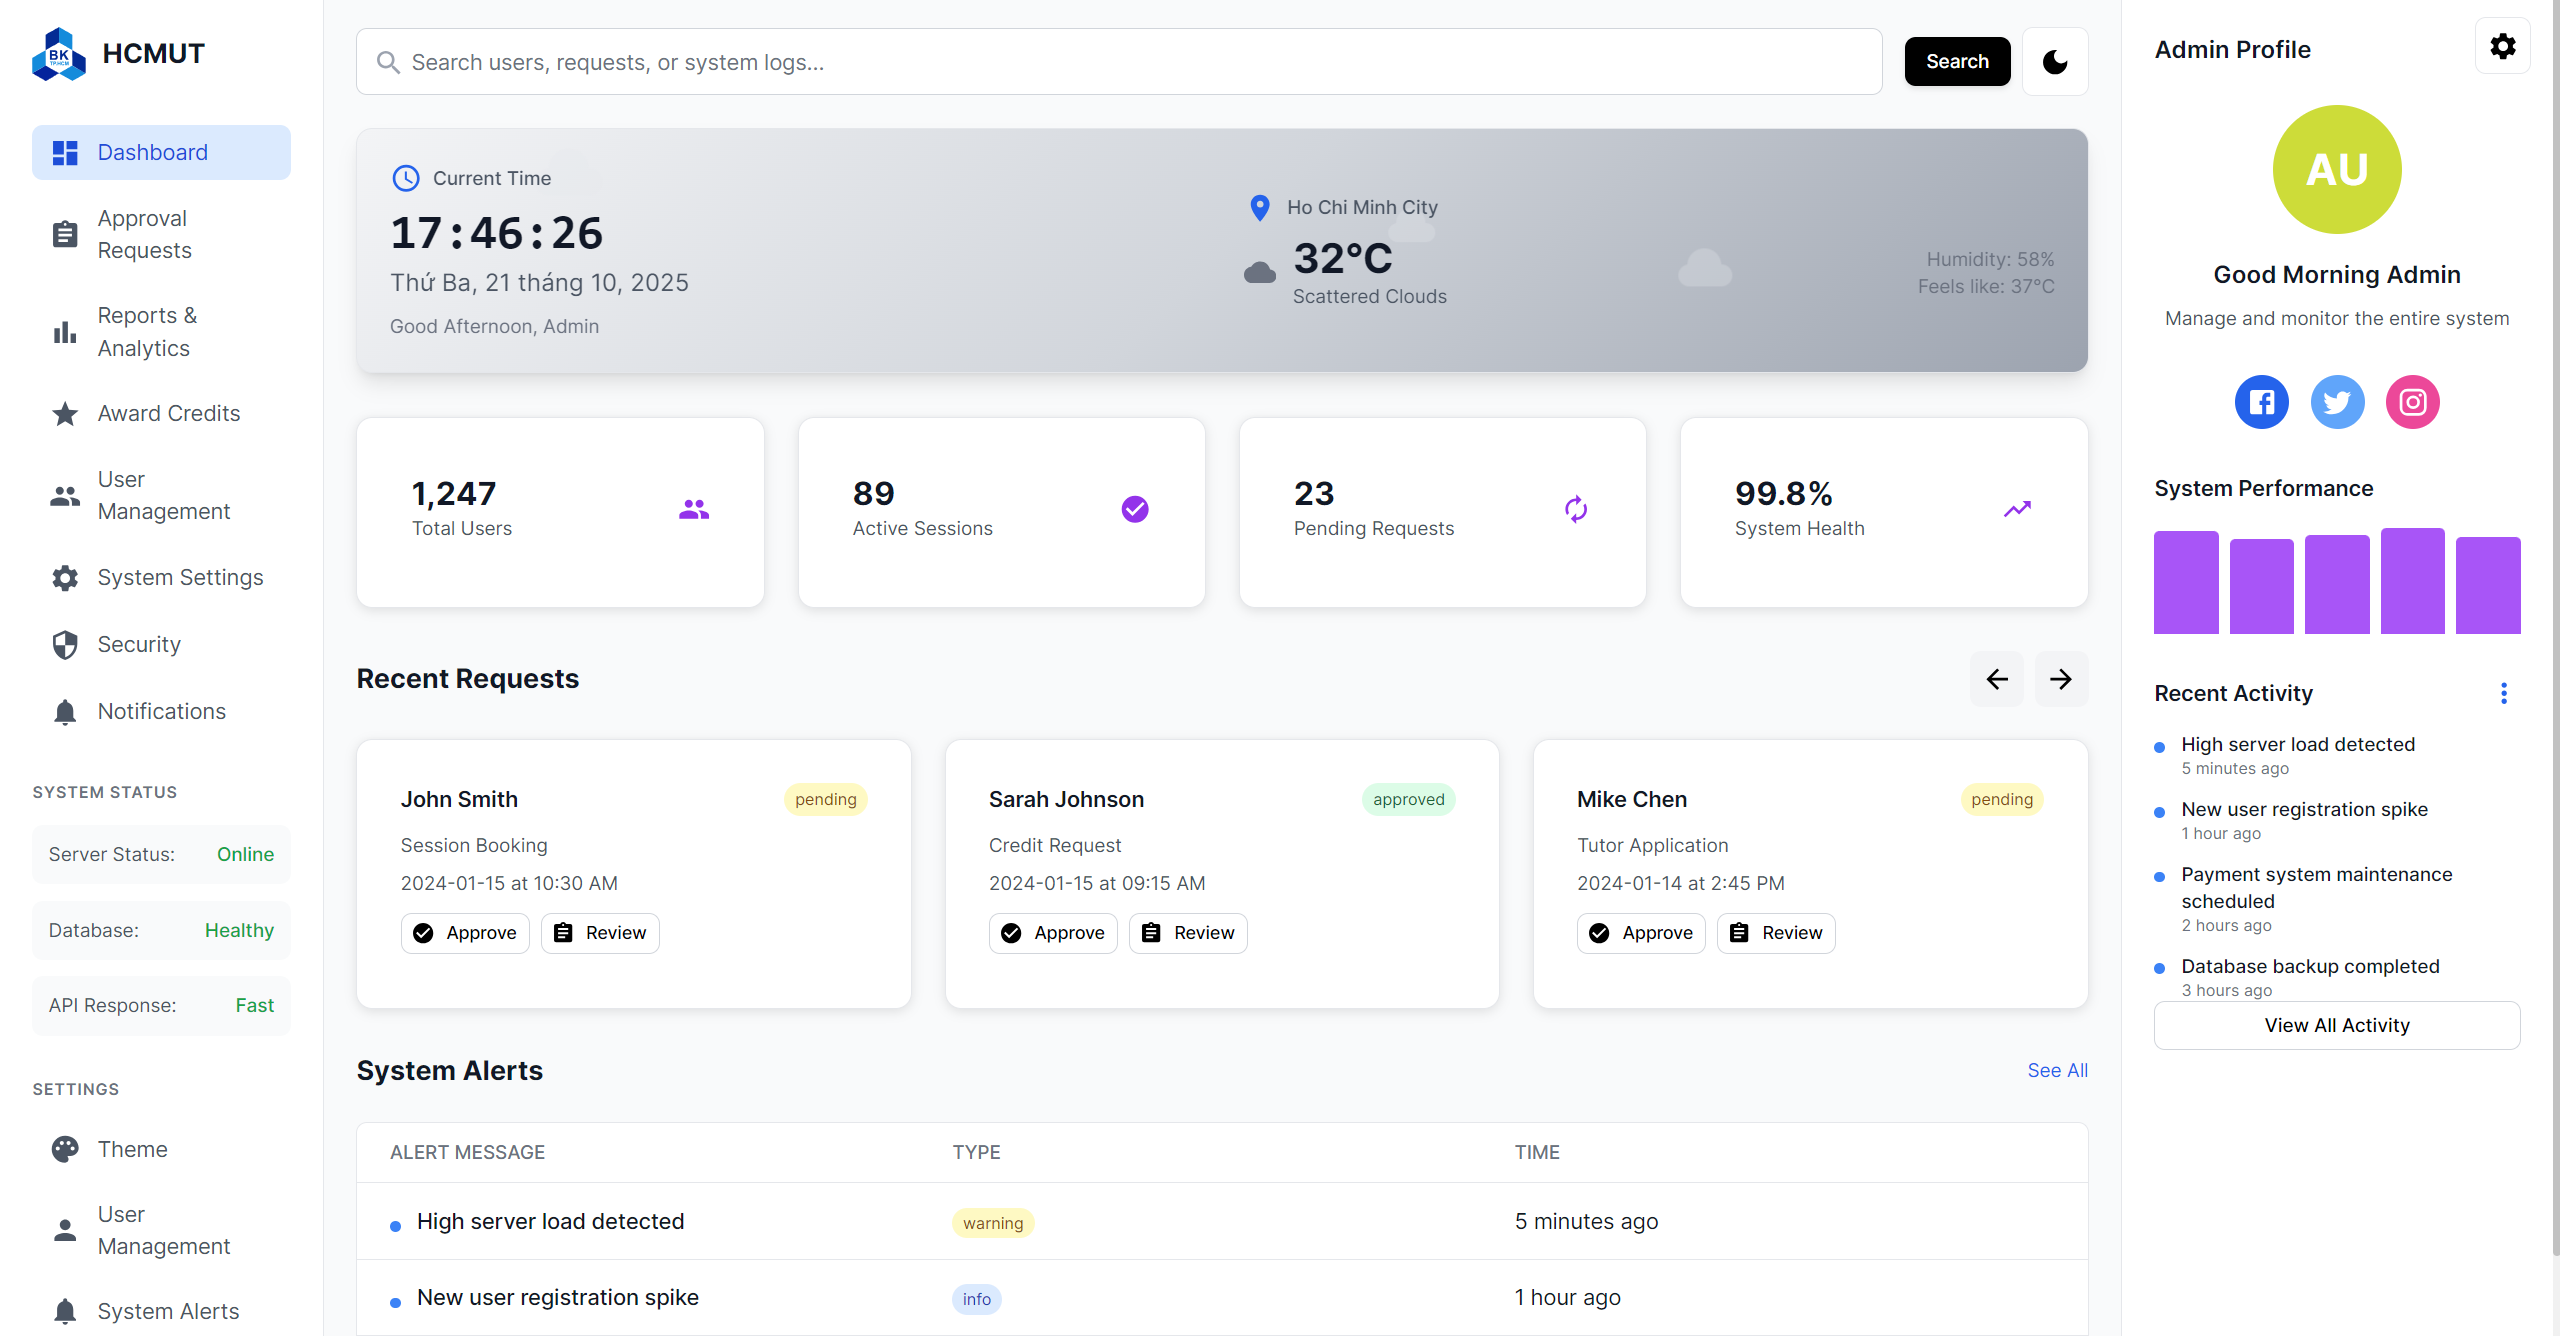
\includegraphics[width=\textwidth]{graphics/chapter2/management/management_dashboard_desktop_overall.png}
    \caption{Management Dashboard Overview (Desktop)}
    \label{fig:management_dashboard_desktop_overall}
\end{figure}

\paragraph{General Overview (Desktop)}
The dashboard features a three-column layout: a left navigation sidebar, a central content area displaying key metrics and operational data, and a right panel for admin profile and recent system activity.

\subsubsection{Approval Requests}

\noindent The "Approval Requests" page provides administrators with an interface to review and manage various user-submitted requests, enabling efficient approval or rejection workflows.

\begin{figure}[H]
    \centering
    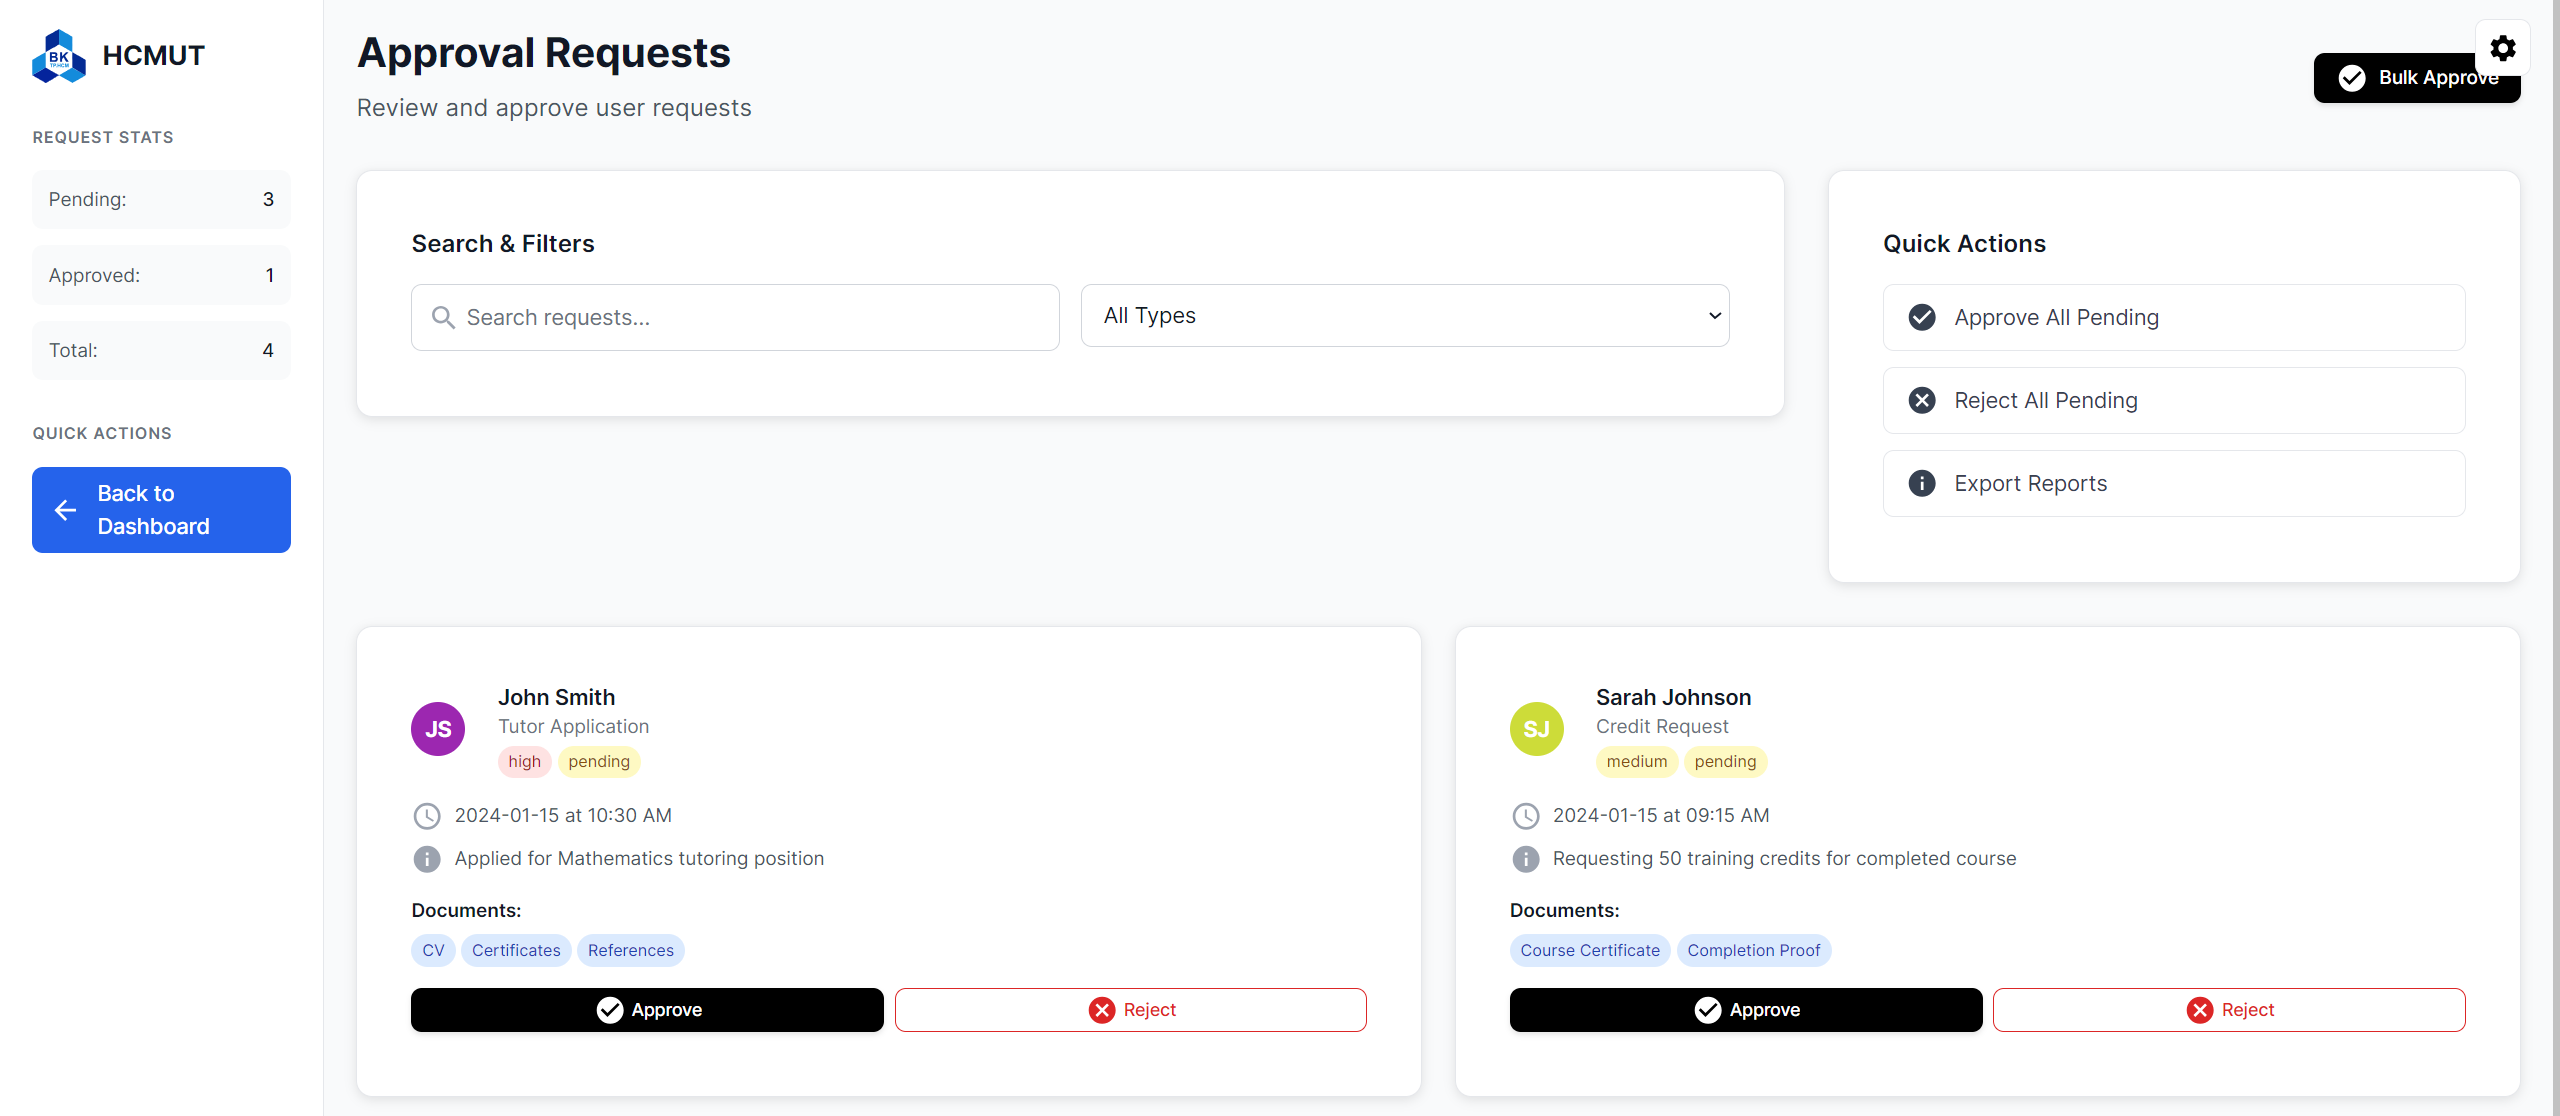
\includegraphics[width=\textwidth]{graphics/chapter2/management/approval_requests_desktop_overall.png}
    \caption{Approval Requests Page Overview (Desktop)}
    \label{fig:approval_requests_desktop_overall}
\end{figure}

\paragraph{General Overview (Desktop)}
The desktop interface features a clean layout with request statistics, search and filter options, bulk action buttons, and individual request cards for efficient management.

\subsubsection{Reports \& Analytics}

\noindent The "Reports \& Analytics" page provides administrators with comprehensive insights into system performance, user engagement, and key metrics through visual reports and data analysis tools.


\begin{figure}[H]
    \centering
    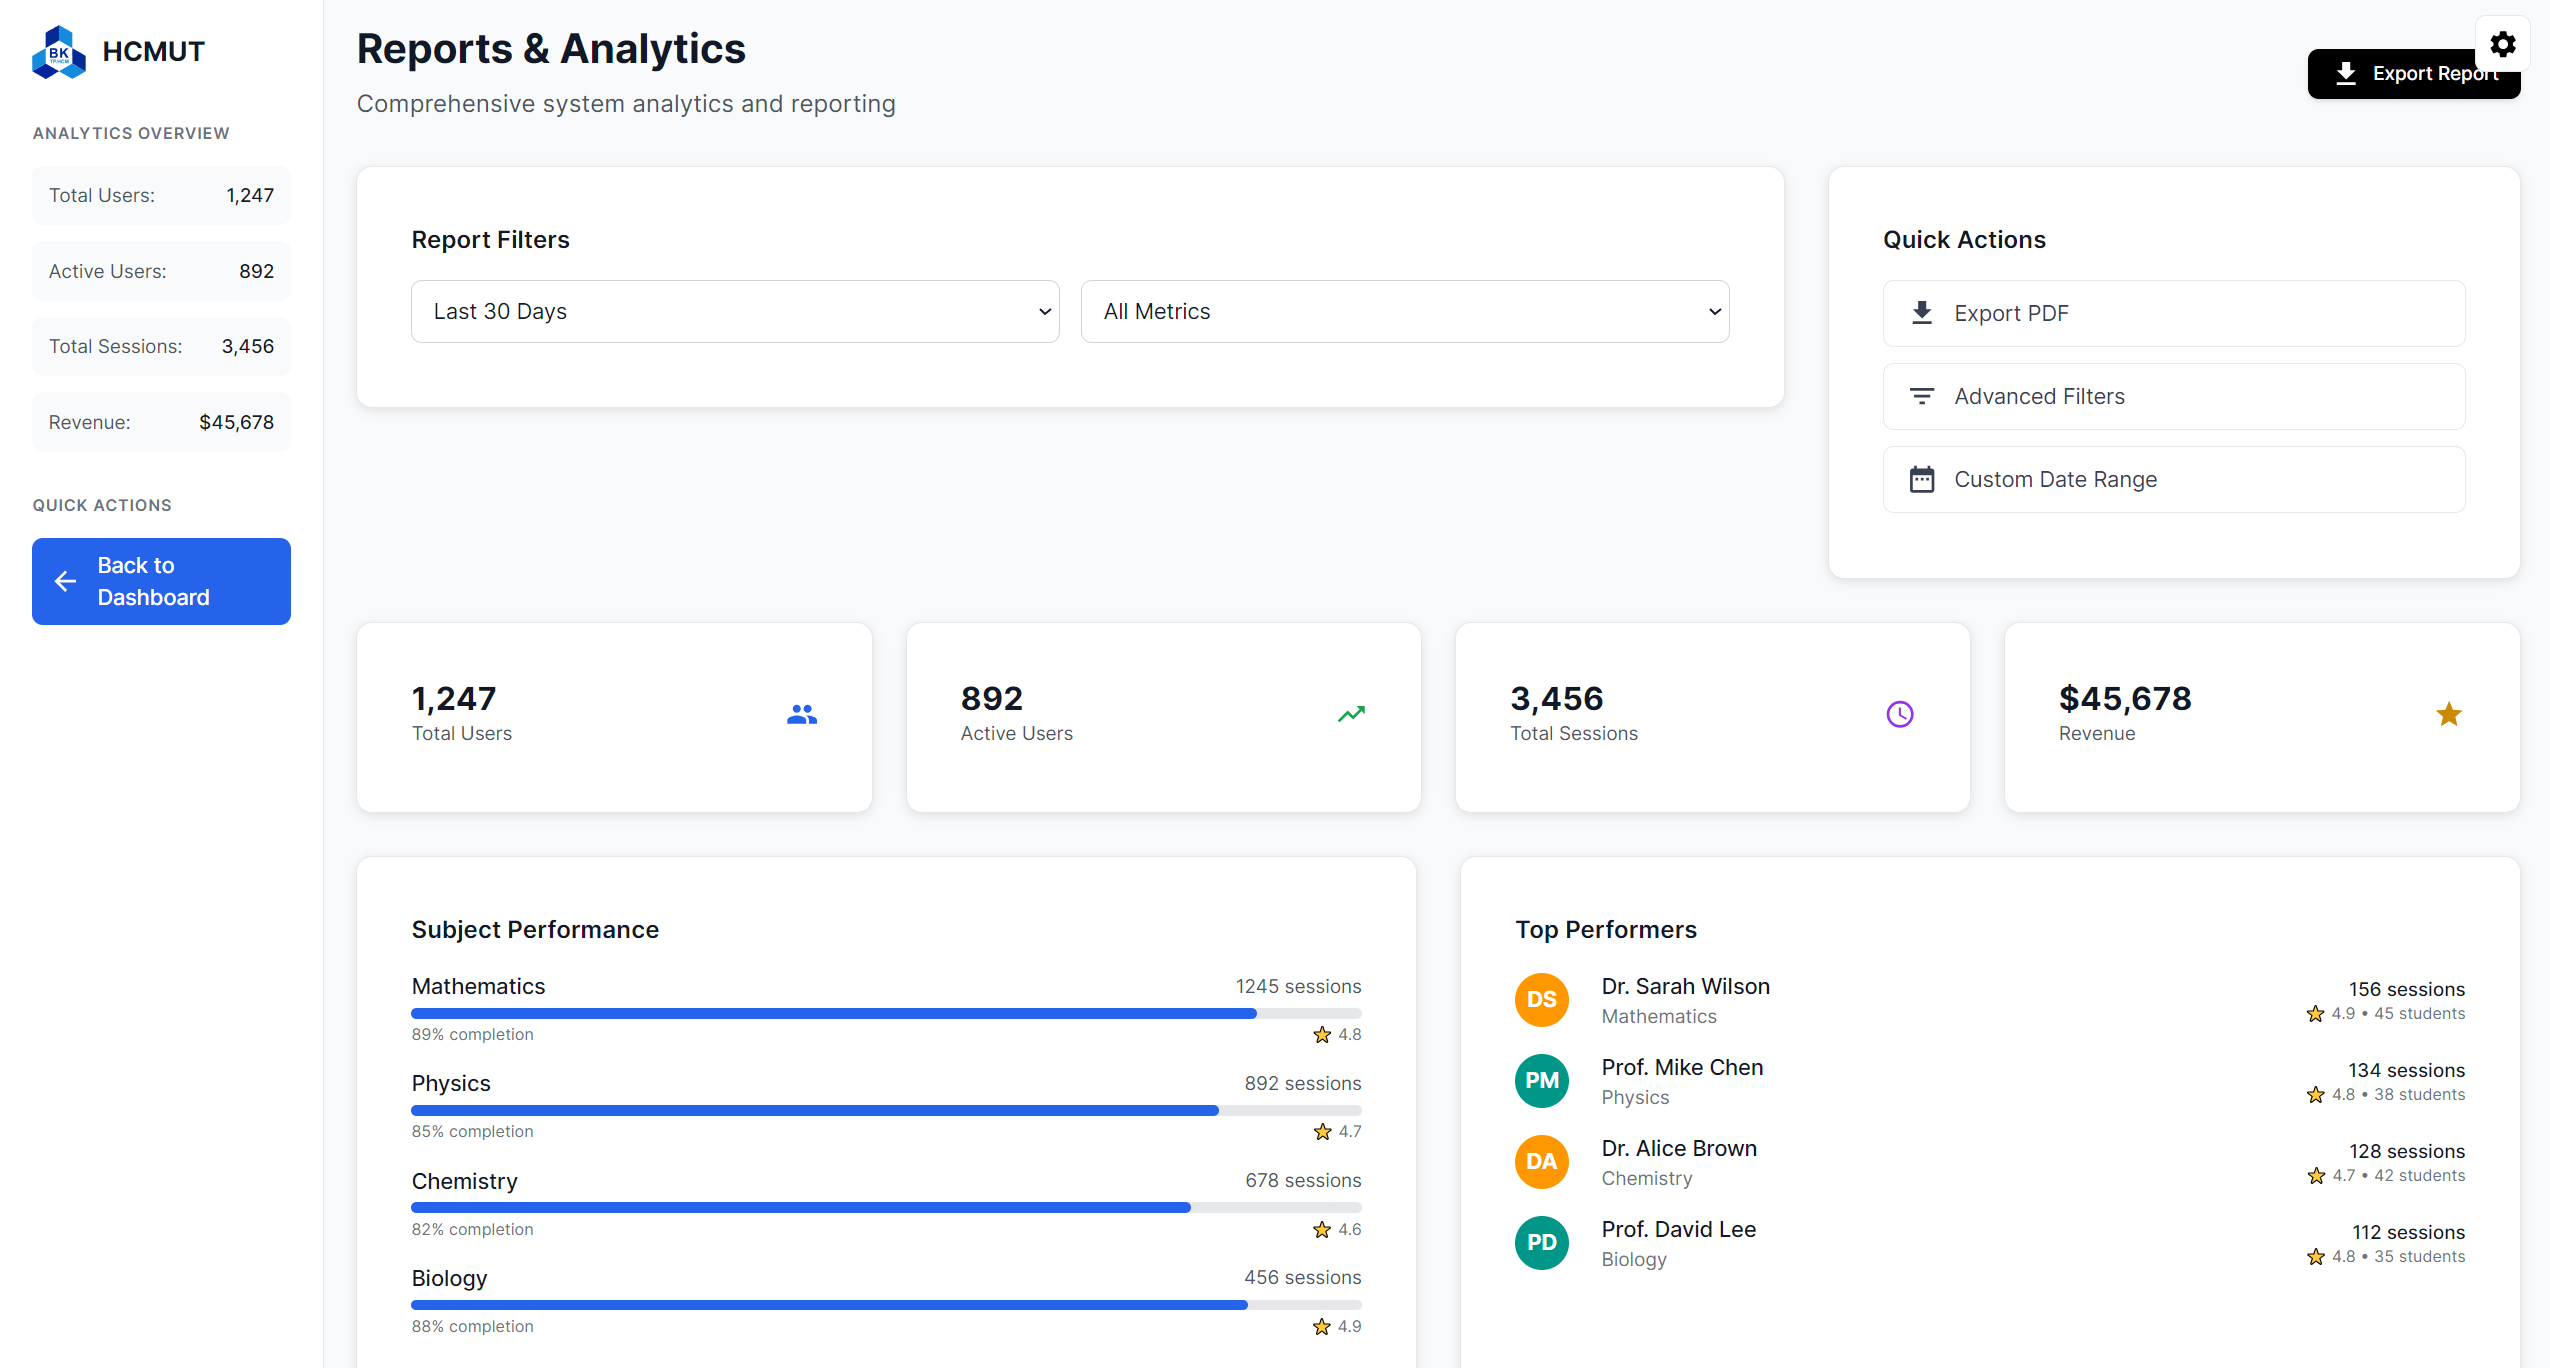
\includegraphics[width=\textwidth]{graphics/chapter2/management/reports_analytics_desktop_overall.png}
    \caption{Reports \& Analytics Page Overview (Desktop)}
    \label{fig:reports_analytics_desktop_overall}
\end{figure}

\paragraph{General Overview (Desktop)}
The desktop interface features a clean layout with key performance indicators, advanced filtering options, export capabilities, and detailed performance metrics across different subjects and top performers.

\subsubsection{Award Credits}

\noindent The "Award Credits" page provides administrators with a comprehensive interface to manage training credits, view credit statistics, search users, and award credits individually or in bulk.

\begin{figure}[H]
    \centering
    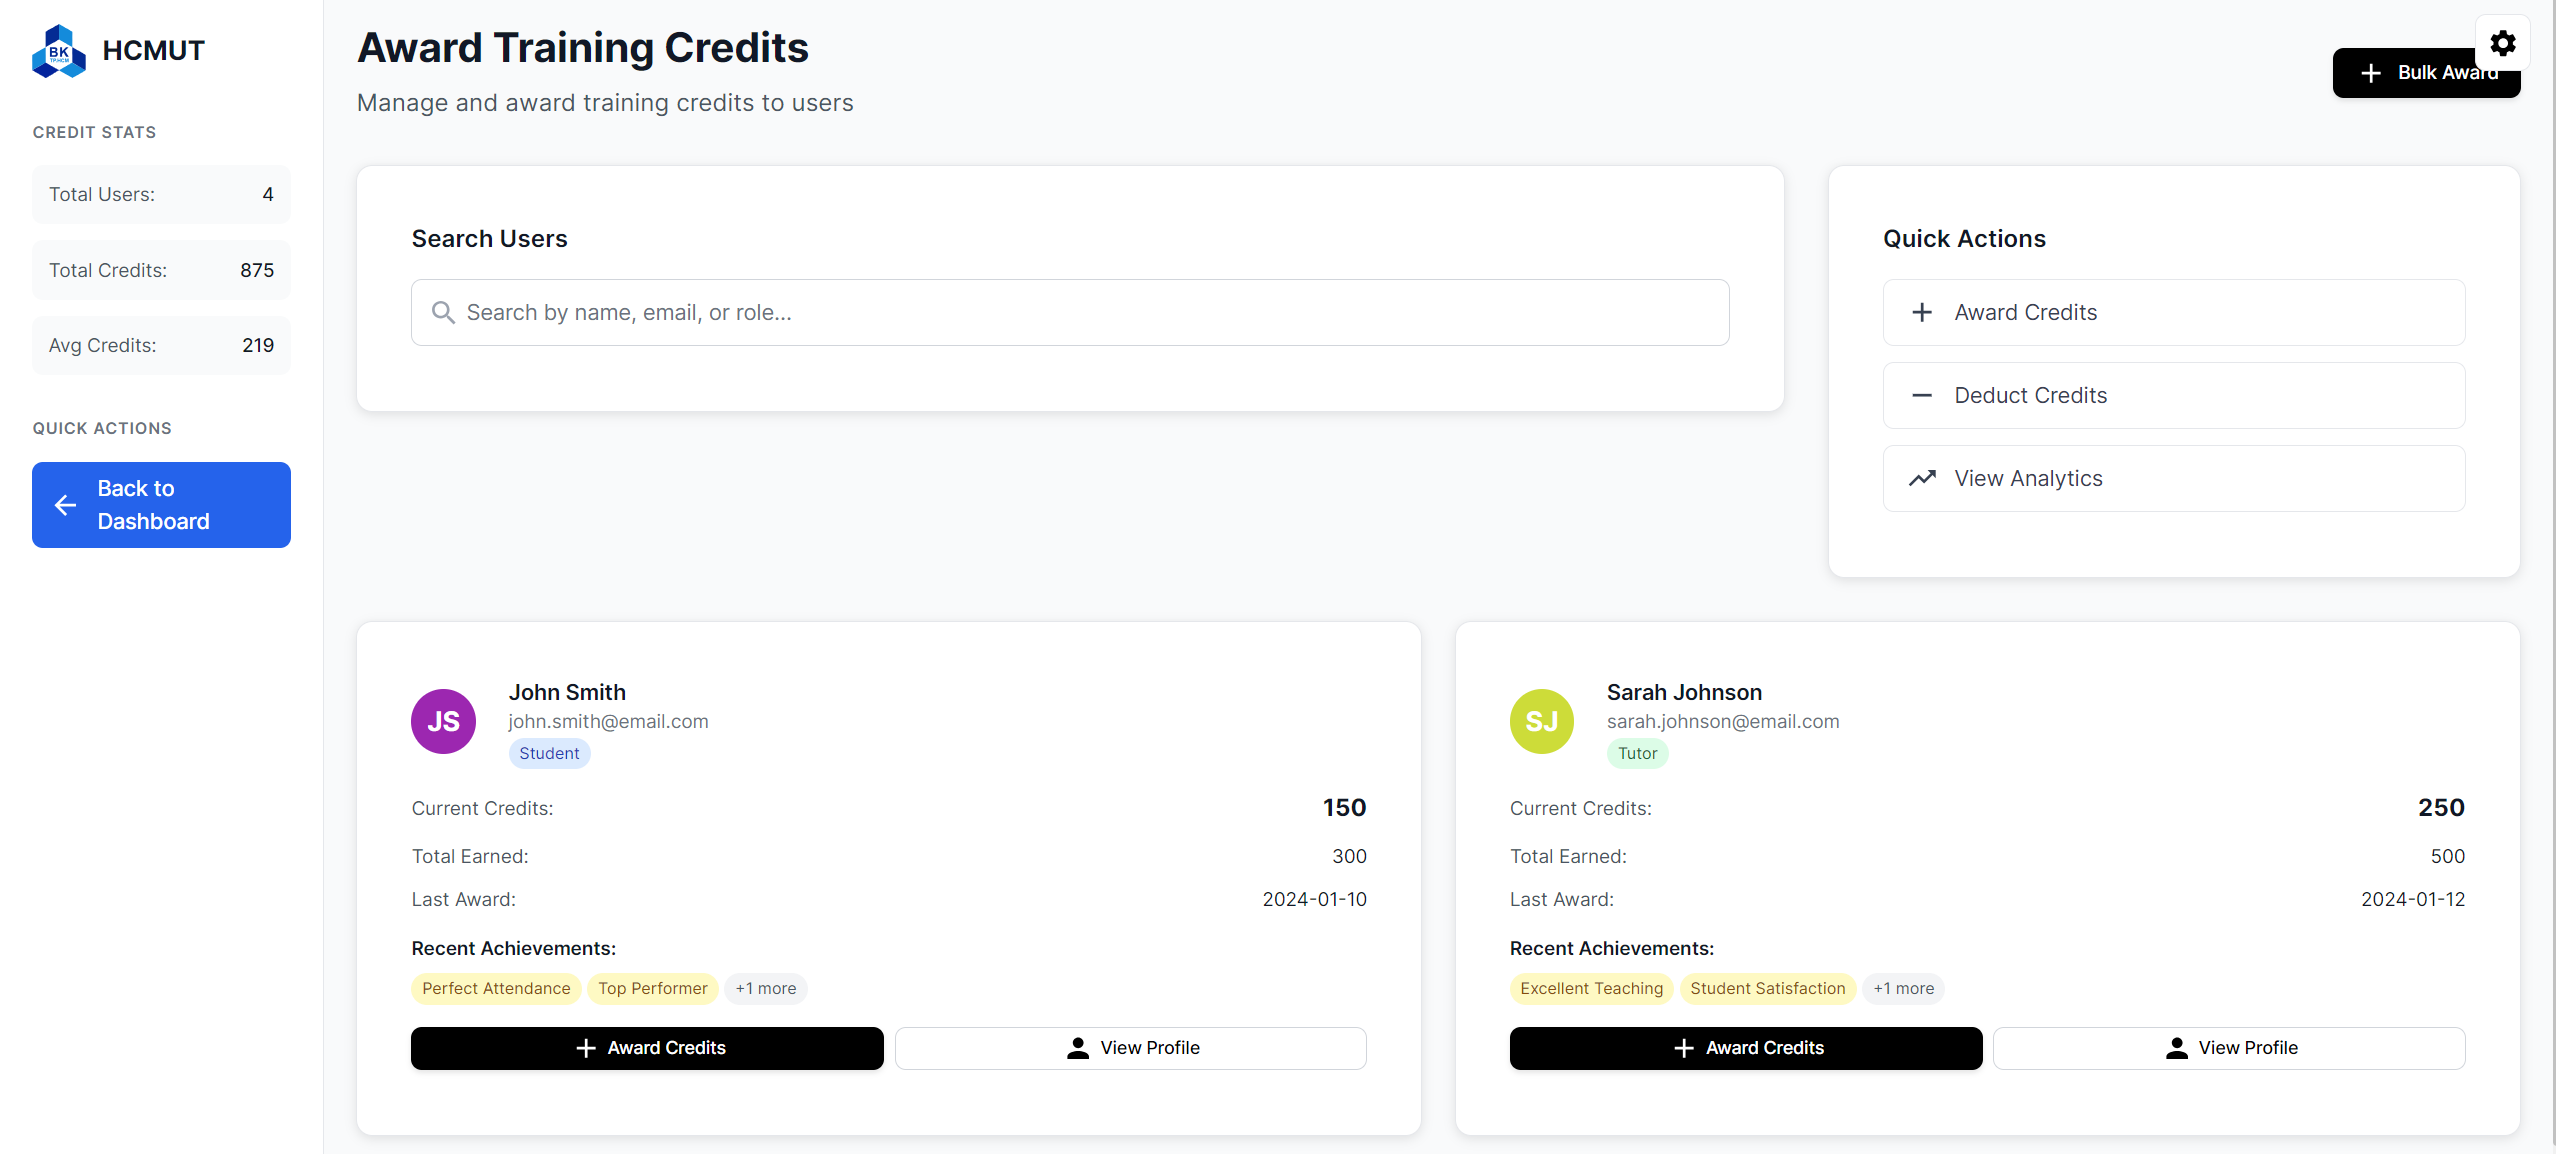
\includegraphics[width=\textwidth]{graphics/chapter2/management/award_credits_desktop_overall.png}
    \caption{Award Credits Page Overview (Desktop)}
    \label{fig:award_credits_desktop_overall}
\end{figure}

\paragraph{General Overview (Desktop)}
The desktop interface features a clean layout with credit statistics, user search and filtering, bulk actions, and individual user credit management cards for efficient credit administration.
